Het grootste probleem bij overlappende schermen is de verloren informatie te recupereren en te reconstrueren. Een gevonden hoek wordt volgens het reconstructie algoritme enkel correct bevonden als hij minstens voldoende dicht bij het middelpunt van het scherm ligt tegenover zijn overstaande hoek. De gebruikte threshold is dat de afstand van een hoek tot het middelpunt minimaal 70 procent van zijn overstaande hoek moet zijn. Als dit niet het geval is zal de puntspiegeling van zijn overstaande hoek gebruikt worden.
Om te testen of deze verhouding en puntspiegeling stand houdt onder verschillende omstandigheden, zijn er in het 3D-software pakket Blender scenes gemaakt om een realistische situatie te creëren. Omdat er gewerkt kan worden met een echte camera en rotatie volgens drie dimensies, kon het algoritme nauwkeurig getest worden. Door de grootte van het scherm en de afstand van de camera tegenover het scherm constant te houden, kon de invloed van de rotatie van het scherm en de focal length van de camera als variabele ingesteld worden om zo telkens de resultaten van het reconstructie algoritme te testen. De testreeksen werden verdeeld als volgt: per focal length werd het scherm van 0 to 90 graden per 5 gedraaid. Omdat de meest voorkomende smartphone cameras een focal lenght hebben van 25mm tot 35mm werd de focal length getest van 20mm tot 40mm met een stap van 2mm. Er werden dus in totaal 180 beelden gemaakt en getest.
De resultaten liggen niet al te ver af van de verwachtingen. Het algoritme houdt zeer goed stand bij relatief kleine kleine vervormingen door de focal length, zeker omdat de kleinst geteste focal length van 20mm wel wat kleiner is dan de de gemiddelde camera. Als het scherm weg begint te draaien geeft het reconstructie algoritme vaak een reconstructie waar er eigenlijk geen nodig is. Dit gebeurde gemiddeld rond de 60 tot 65 graden. Dit is waar een enkele threshold te kort schiet om een onderscheid te maken of het scherm niet volledig zichtbaar is, of relatief scherp gedraaid.

\begin{figure}

	\center
	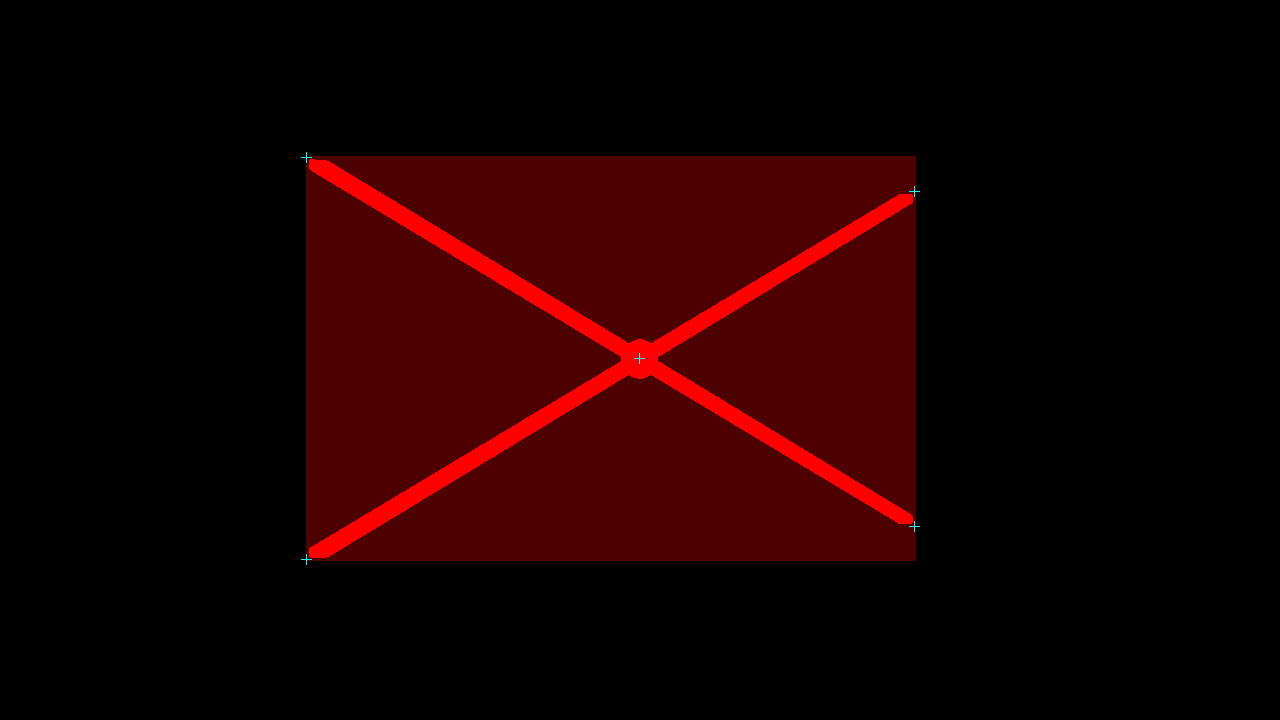
\includegraphics[width=0.4\textwidth]{correct-resultaat}
	\caption{Correct resultaat}
	\label{corr}
\end{figure}

\begin{figure}

	\center
	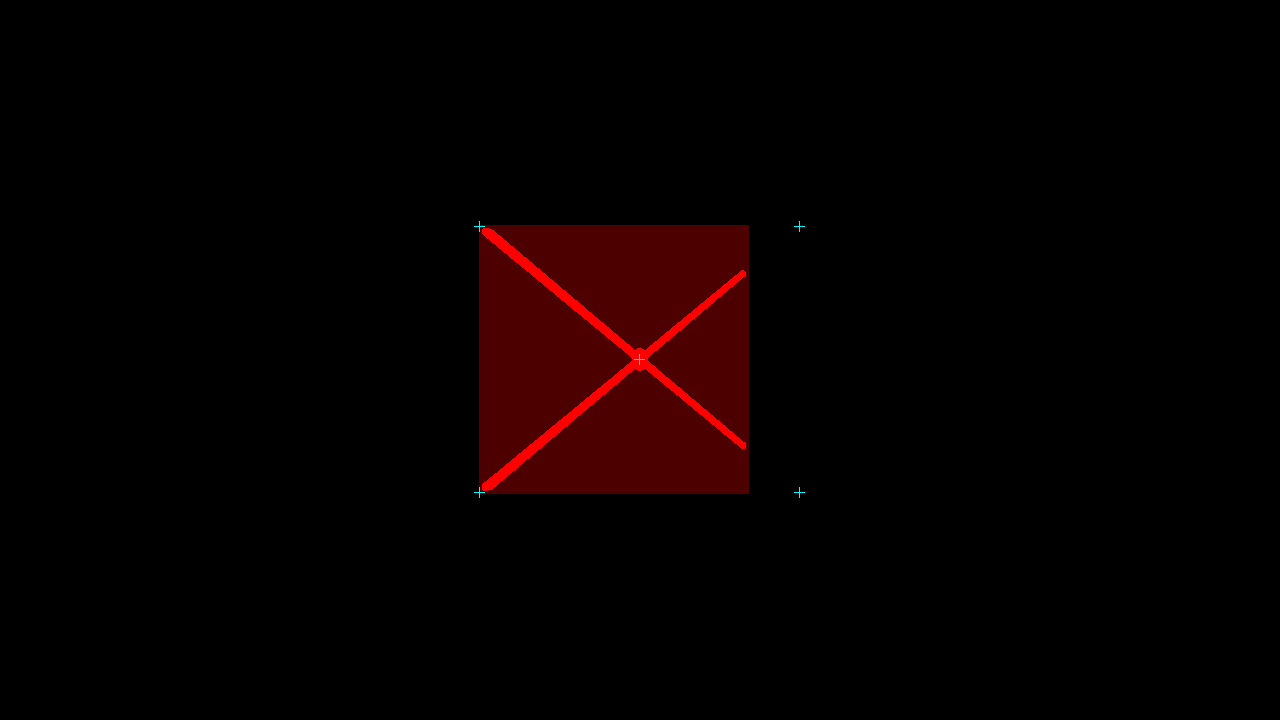
\includegraphics[width=0.4\textwidth]{fout-resultaat}
	\caption{Foute reconstructie}
	\label{fout}
\end{figure}